\documentclass[a4j,12pt,]{jarticle}
 \usepackage{float}
 \usepackage{siunitx} %%SI単位系用
 \usepackage{amssymb, amsmath}
 \usepackage{ascmac,here,txfonts}
 \usepackage{hyperref}
 \usepackage{listings}
 \usepackage{pxjahyper}
 \usepackage[dvipdfmx]{graphicx}
 \usepackage{amssymb, amsmath}
  \usepackage{listings}
  \usepackage[dvipdfmx]{color}
 
 \lstset{
   language={Python},
   basicstyle={\ttfamily},
   identifierstyle={\small},
   commentstyle={\small\itshape},
   keywordstyle={\small\bfseries},
   ndkeywordstyle={\small},
   stringstyle={\small\ttfamily},
   frame={single},
   breaklines=true,
   columns=[l]{fullflexible},
   numbers=left,
   xrightmargin=0zw,
   xleftmargin=3zw,
   numberstyle={\scriptsize},
   stepnumber=1,
   numbersep=1zw,
   lineskip=-0.5ex,
 }
\begin{document}

{\noindent\small 第17回報告書 \hfill\today}
\begin{center}
  {\Large ElasticSearchサーバーのCO\textsubscript{2}データの移行について}
\end{center}
\begin{flushright}
  祖父江匠真 \\
\end{flushright}

\section{概要}
今回は, 133.71.201.197から133.71.106.141へのElasticSearchサーバー間のCO\textsubscript{2}データの移行後に発生したラズベリーパイからデータのインサートが出来ない問題への対応と, 移行元ElasticSearchサーバーから移行されていないCO\textsubscript{2}データの移行について報告する.

\section{ラズベリーパイからデータのインサートが出来ない問題について}

私が実装したデータ移行プログラムを使用して作成したElasticSearchのインデックスに対してラズベリーパイからデータのインサートが出来ない問題が発生した.

そこで, インデックスの作成を私のデータ移行プログラム上からではなく, 高木君側で行ってもらい, ラズベリーパイから正常にデータのインサートが出来ていることを確認した上で, 私が実装したデータ移行プログラムを使用してCO\textsubscript{2}データの移行を行うことで問題を解決した.

\section{移行元ElasticSearchサーバーから移行されていないCO\textsubscript{2}データの移行について}

私が実装したデータ移行プログラムを使用して133.71.201.197から133.71.106.141のElasticSearchサーバーへCO\textsubscript{2}データを移行したのが2023年5月中旬頃であり, 高木君が, 移行先である133.71.106.141のElasticSearchサーバーに対してラズベリーパイからCO\textsubscript{2}データのインサートを行うよう対応したのが2023年7月中旬であったため, 2023年5月中旬から2023年7月中旬までの間の約2ヶ月間のCO\textsubscript{2}データが移行先のElasticSearchサーバーに移行出来ていなかった. そこで, 追加の移行作業を行った.

移行方法は以下のとおりである.

\begin{enumerate}
  \item まず, 2023年5月中旬に移行した際の全移行データの中で最も最新のutctimeフィールドの値を検索する.
  \item 次に, 移行先ElasticSearchサーバーに対してラズベリーパイからインサートされた全データの中で最も古いutctimeフィールドの値を検索する.
  \item elasticdump \cite{1}ライブラリを使用して, 2023年5月1日0時0分0秒以降のutctimeを持つドキュメントを, 移行元ElasticSearchサーバーのインデックス名にco2という文字列を含むインデックスからローカルマシンにエクスポートする.
  \item 部屋番号(number)とタイムスタンプ(JPtime)の組み合わせがユニークになるようにエクスポートしたデータをフィルタリングする.
  \item 更に, 1と2で得られたutctimeの範囲に含まれるutctimeを持つドキュメントのみになるようフィルタリングする.
  \item フィルタリング後のデータを移行先ElasticSearchサーバーにバルクインサートする.
\end{enumerate}

\section{kibanaによるデータの可視化}

2023年5月中旬から2023年7月中旬までの間の約2ヶ月間のCO\textsubscript{2}データを移行した後のco2\_modbusインデックスについて, 横軸をタイムスタンプ(utctime)とし, 縦軸をPPM, RH, TEMPとしてそれぞれプロットしたものを図 \ref{p1} 〜 図 \ref{p3}に示す.

\begin{figure}[H]
  \begin{center}
    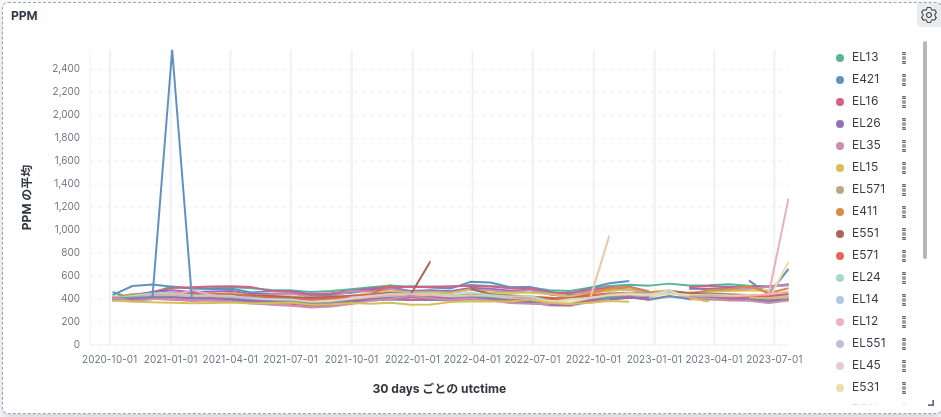
\includegraphics[width=160mm]{ppm.png}
    \caption{co2\_modbusのPPM}
    \label{p1}
  \end{center}
\end{figure}

\begin{figure}[H]
  \begin{center}
    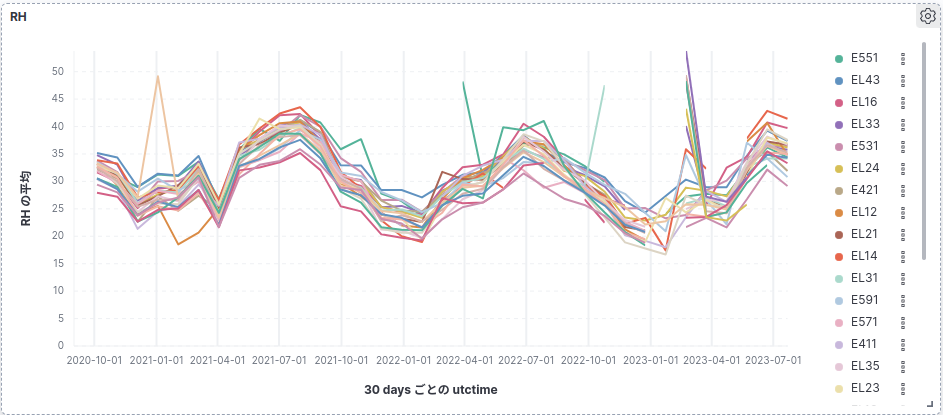
\includegraphics[width=160mm]{rh.png}
    \caption{co2\_modbusのRH}
    \label{p2}
  \end{center}
\end{figure}

\begin{figure}[H]
  \begin{center}
    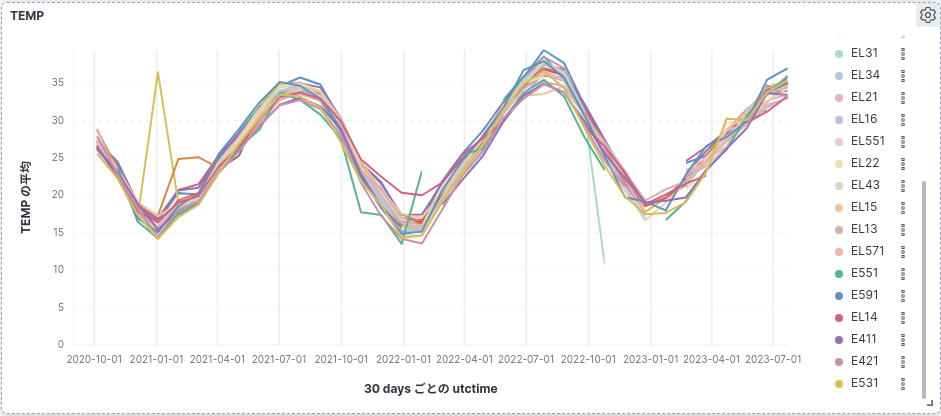
\includegraphics[width=160mm]{temp.png}
    \caption{co2\_modbusのTEMP}
    \label{p3}
  \end{center}
\end{figure}

今回, 追加でCO\textsubscript{2}データを移行した2023年5月中旬から2023年7月中旬までの期間において, 図 \ref{p1} 〜 図 \ref{p3}より, 連続的にデータが変化していることが目視で確認できるので, データ移行は正常に出来たと判断できる.

\section{まとめ}
今回は, 133.71.201.197から133.71.106.141へのElasticSearchサーバー間のCO\textsubscript{2}データの移行後に発生したラズベリーパイからデータのインサートが出来ない問題を解決したことと, 移行元ElasticSearchサーバーから移行されていないCO\textsubscript{2}データの移行を行い, kibanaを使ってデータ移行が正常に出来たことを報告した.

次回は, 133.71.201.197のElasticSearchサーバーにあるpcs\_recyclekanという名前のインデックス以外のインデックスについて調査を行い, 必要であればデータ移行を行う.

\begin{thebibliography}{5}
  \bibitem{1}Ferron H, ”ElasticDump”, https://github.com/elasticsearch-dump/elasticsearch-dump, 参照 June 19,2023.
\end{thebibliography}

\end{document}

